\documentclass[]{article}
\usepackage{lmodern}
\usepackage{amssymb,amsmath}
\usepackage{ifxetex,ifluatex}
\usepackage{fixltx2e} % provides \textsubscript
\ifnum 0\ifxetex 1\fi\ifluatex 1\fi=0 % if pdftex
  \usepackage[T1]{fontenc}
  \usepackage[utf8]{inputenc}
\else % if luatex or xelatex
  \ifxetex
    \usepackage{mathspec}
  \else
    \usepackage{fontspec}
  \fi
  \defaultfontfeatures{Ligatures=TeX,Scale=MatchLowercase}
\fi
% use upquote if available, for straight quotes in verbatim environments
\IfFileExists{upquote.sty}{\usepackage{upquote}}{}
% use microtype if available
\IfFileExists{microtype.sty}{%
\usepackage{microtype}
\UseMicrotypeSet[protrusion]{basicmath} % disable protrusion for tt fonts
}{}
\usepackage[margin=1in]{geometry}
\usepackage{hyperref}
\hypersetup{unicode=true,
            pdftitle={Valuing information for conservation and natural resource management: a review},
            pdfauthor={William K. Morris},
            pdfborder={0 0 0},
            breaklinks=true}
\urlstyle{same}  % don't use monospace font for urls
\usepackage{natbib}
\bibliographystyle{voiReview.bst}
\usepackage{longtable,booktabs}
\usepackage{graphicx,grffile}
\makeatletter
\def\maxwidth{\ifdim\Gin@nat@width>\linewidth\linewidth\else\Gin@nat@width\fi}
\def\maxheight{\ifdim\Gin@nat@height>\textheight\textheight\else\Gin@nat@height\fi}
\makeatother
% Scale images if necessary, so that they will not overflow the page
% margins by default, and it is still possible to overwrite the defaults
% using explicit options in \includegraphics[width, height, ...]{}
\setkeys{Gin}{width=\maxwidth,height=\maxheight,keepaspectratio}
\IfFileExists{parskip.sty}{%
\usepackage{parskip}
}{% else
\setlength{\parindent}{0pt}
\setlength{\parskip}{6pt plus 2pt minus 1pt}
}
\setlength{\emergencystretch}{3em}  % prevent overfull lines
\providecommand{\tightlist}{%
  \setlength{\itemsep}{0pt}\setlength{\parskip}{0pt}}
\setcounter{secnumdepth}{5}

%%% Use protect on footnotes to avoid problems with footnotes in titles
\let\rmarkdownfootnote\footnote%
\def\footnote{\protect\rmarkdownfootnote}

%%% Change title format to be more compact
\usepackage{titling}

% Create subtitle command for use in maketitle
\newcommand{\subtitle}[1]{
  \posttitle{
    \begin{center}\large#1\end{center}
    }
}

\setlength{\droptitle}{-2em}
  \title{Valuing information for conservation and natural resource management: a
review}
  \pretitle{\vspace{\droptitle}\centering\huge}
  \posttitle{\par}
  \author{William K. Morris}
  \preauthor{\centering\large\emph}
  \postauthor{\par}
  \predate{\centering\large\emph}
  \postdate{\par}
  \date{2017-09-20}

\usepackage{titlesec}
\titleformat{\paragraph}{\small\normalfont\bfseries}{}{0pt}{}
\titleformat{\subparagraph}{\small\normalfont}{}{0pt}{}
\linespread{2}\selectfont
\usepackage{booktabs}
\usepackage{setspace}
\usepackage{caption}
\usepackage{tikz}
\usepackage{pdflscape}
\captionsetup{font={stretch=2}}
\usepackage{pbox}
\usepackage{tabu}
\usepackage[displaymath,mathlines]{lineno}
\linenumbers

\usepackage{amsthm}
\newtheorem{theorem}{Theorem}[section]
\newtheorem{lemma}{Lemma}[section]
\theoremstyle{definition}
\newtheorem{definition}{Definition}[section]
\newtheorem{corollary}{Corollary}[section]
\newtheorem{proposition}{Proposition}[section]
\theoremstyle{definition}
\newtheorem{example}{Example}[section]
\theoremstyle{definition}
\newtheorem{exercise}{Exercise}[section]
\theoremstyle{remark}
\newtheorem*{remark}{Remark}
\newtheorem*{solution}{Solution}
\begin{document}
\maketitle


\subsection*{Abstract}\label{abstract}
\addcontentsline{toc}{subsection}{Abstract}

In conservation and natural resource management, scientist and practitioners have begun to realize the importance of valuing information. Information has a central role to play when it comes to making good decisions that will benefit the environment and satisfy management objectives. But there are limits to benefits from more information. Key questions for practitioners are: how much information is warranted for decision making? What kind of information? And what level of certainty is enough before a decision can be made with confidence in the outcome? These questions arise as the information itself comes at some cost. This cost must be weighed against the value of information for the decision at. Decision theoretic tools aimed at information valuing have existed for over half a century but only relatively recently have begun to appear in the conservation and natural resource management literature. Here, we examine a suite of case studies employing value of information (VOI) analyses to applied ecological decision problems. We have surveyed case studies using VOI analysis in the strict sense and compare and contrast them to less formal methods that also, sometimes inadvertently, put a value on ecological data in the context of decision making. Our aim here, is to provide an overview of the use of VOI in the field to date and to glean generalities. We found that the two strands of information valuing, formal and informal, have their own distinct characteristics and the casual reader of either may get a different picture about the value of information if they were only to engage with one or the other. Formal VOI analyses tend to report a low value of information, while informal methods often report larger values. We conjecture that biases stemming from the way that case studies are performed and selected may account for this discrepancy. A feature common to both approaches is that the cost of information is rarely calculated or reported. For greater insight into any generalities on information valuing, future work in conservation sciences should place greater emphasis on information cost and converting costs into the same currency as decision objectives.

\subsection*{Introduction}\label{introduction}
\addcontentsline{toc}{subsection}{Introduction}

A value of information (VOI) theory was outlined over half a century ago
\citep{Raiffa1961}. But only relatively recently has it begun to be used
within the field of conservation and natural resource management. Here
we review the recent literature on valuing information for conservation
and natural resource management. We classify information valuing by the
type of decisions being made and the type of information being learned.
Our literature analysis aims to provide an overview of the use of VOI in
the field to date, and to glean generalities from the body of work as a
whole. We have attempted to be comprehensive for case studies that
employ VOI analysis in the strict sense, save for examples involving
fisheries management, where the method has a longer and deeper history
\citep[see e.g.,][]{Walters1986} (and including all examples would be
counter-productive). Instead, we have included only a few fisheries
management examples that tend to focus more on biodiversity conservation
rather than the commercial aspects of fisheries
\citep[e.g.,][]{Costello2010}. We also include some case studies that
employ informal or post-hoc information valuing
\citep[e.g.,][]{Balmford1999, Hermoso2013}. We do not claim that these
latter examples are by any means an exhaustive list of this study type,
as lacking a common language to describe the methods used, informal
information valuing studies are difficult to locate in literature
databases.

Before addressing the recent history of information valuing for
conservation and natural resource management we'll first turn to the
origin of the concept and define it in its various forms to a degree
necessary to discuss its application. Information, in the context of VOI
analyses has no value in and of its self. The value of a piece
information arises from its potential to increase the performance of a
decision that the particular information pertains to. It is the
magnitude of this performance increase that constitutes the value of
information. The value of information in this sense, first appeared in
mid 20th century via the seminal work of Raiffa and Schlaifer's Applied
Statistical Decision Theory \citep{Raiffa1961}. For an introduction to
the subject and it's theoretical underpinnings the reader need go no
further. The logic of VOI analyses has evolved little since this early
work and it is mainly in the algorithms used to calculate it, for its
various applications, that advances have been made
\citep{Yokota2004a, Yokota2004b}.

Strictly speaking the \emph{value} of information cannot be
foreseen---to do so, a decision would need to be made both with and
without the information and the performance compared. Even if it were
possible it would not be very useful, as it would not inform the
decision maker about the worth of seeking new information prior to
decision making. To be useful, the value of information must come in the
form of an expected value. An expected value being the performance a
decision maker expects to get from a particular action. That expectation
being the average of all possible outcomes weighted by their respective
probabilities of happening. The value of information is therefore
typically encountered as an \emph{expected value} of information (EVI).

\subsection*{Types of VOI}\label{types-of-voi}
\addcontentsline{toc}{subsection}{Types of VOI}

Here we attempt to classify VOI as it has been practised to date in the
conservation sciences. Broadly, information valuing falls into two
types, informal and formal. The latter is any VOI analyses employing the
formal methods outlined by the decision theoretic toolset we discuss
further below. But this is by no means the only way to think about,
calculate and report the value of information.

\subsubsection*{Informal VOI}\label{informal-voi}
\addcontentsline{toc}{subsubsection}{Informal VOI}

Many authors have undertaken informal VOI analyses, in which they arrive
at what is conceptually a calculation of the value of information, even
though they don't arrive there by the conventional means. More often
than not, these informal value of information analyses take the form of
post-hoc comparisons of decision outcomes with different datasets that
represent varied levels of uncertainty. The use of informal VOI analyses
is particularly prevalent in the field of spatial conservation planning
\citep[e.g.,][]{Balmford1999}. Most examples of informal VOI fall in
this category of decision problem.

\paragraph*{Comparisons of data
quantity}\label{comparisons-of-data-quantity}
\addcontentsline{toc}{paragraph}{Comparisons of data quantity}

Some informal VOI analyses compare datasets, or data subsets, with
different sample-sizes
\citep[e.g.,][]{Grantham2008, Grantham2009, Hermoso2013}. These authors
present case-studies in which they evaluate the same decision problem
using datasets of varying size or a single dataset that has been
subsetted with different sample-sizes in each subset. In these examples,
they arrive at a value of information based on the difference in the
outcome of decision-making with a smaller dataset compared to a larger
dataset. For example, \citet{Hermoso2013} found the performance of
reserve system would improve by up to 230\% when using their full
dataset of fish distributions, compared with any given subsample with a
sample size 15\% of the sample-size of their full dataset.

\paragraph*{Comparisons of data
quality}\label{comparisons-of-data-quality}
\addcontentsline{toc}{paragraph}{Comparisons of data quality}

Another type of post-hoc VOI analysis compares data with more
qualitative differences. The authors of these studies ascribe the
different quality data sources as having greater or less precision and
thus producing more or less uncertain predictions for decision making.
They then proceed the same way as above and evaluate a single decision
problem using the multiple data sources. For example, \citet{Stoms2011}
found that using higher quality information in the design of a
conservation easement scheme in California, resulted in benefits 20
times greater than using a minimal dataset.

The problem with these types of VOI analysis, typically found in the
spatial conservation planning literature, is that in calculating a
post-hoc value of information, they are performing the calculation when
it is too late. While it is interesting to show, after the fact, that
collecting some dataset was worthwhile, it is more important to show
that information has some worth prior to it being collected. To a
certain extent, these studies may be setting up a straw man.

\paragraph*{Active vs.~passive adaptive
management}\label{active-vs.passive-adaptive-management}
\addcontentsline{toc}{paragraph}{Active vs.~passive adaptive management}

There are other examples of informal value of information that don't use
a post-hoc approach to value information. By comparing the expected
outcomes of active vs passive adaptive management
\citep[e.g.,][]{Moore2010, Baxter2011} some sense of the value of
learning can be gleaned without employing the VOI analysis in the strict
sense. We won't explore these ideas further here, other than to note
that this line of enquiry is interesting but none-the-less beyond the
scope of the present work.

\subsubsection*{Formal VOI}\label{formal-voi}
\addcontentsline{toc}{subsubsection}{Formal VOI}

As alluded to above, in formal value of information analyses the
quantity of interest comes in the form of an expected value, the EVI.
The EVI comes in different forms but common to all is that they
represent the performance increase expected when going from optimal
decision making under uncertainty to optimal decision making under less
uncertainty \citep{Yokota2004b}. The concept doesn't stipulate how much
uncertainty there is at either point, just that the latter is less
uncertain than the former.

\subsubsection*{Components of EVI}\label{components-of-evi}
\addcontentsline{toc}{subsubsection}{Components of EVI}

Being the result of a difference, EVI has two components: the expected
value with original information (EVWOI) and the expected value with new
information (EVWNI) where,

\begin{equation}
\mathrm{EVI} = \mathrm{EVWNI} - \mathrm{EVWOI}
\label{eq:EVI}
\end{equation}

The EVWOI is the component common to all forms of EVI as it the expected
value of making a decision under uncertainty without any new
information. Calculating EVWOI involves maximizing the expected value of
decision making under uncertainty, or more formally,

\begin{equation}
\mathrm{EVWOI} = \mathrm{max}_a\mathrm{E}_s[{v(a, s)}]
\label{eq:EVWOI}
\end{equation}

where \(s\) represents the model describing the uncertainty, and \(a\)
represents the actions available to the decision maker. Working from the
inside out, \(v(a,s)\) is the value attained when taking an action,
\(a\), when the model state, \(s\), is at particular point in the space
of its uncertainty. Then, \(\mathrm{E}_s[{v(a, s)}]\) is the expected
value of taking any, \(a\) action accounting for the uncertainty in
\(s\). And finally, \(\mathrm{max}_a\mathrm{E}_s[{v(a, s)}]\) is the
value attained when the action is chosen such that
\(\mathrm{E}_s[{v(a, s)}]\) is maximized.

The EVWNI, on the other hand, varies in form, depending on the
particular form of EVI being calculated. It is to those different forms
of EVI we now turn.

\paragraph*{Forms of EVI}\label{forms-of-evi}
\addcontentsline{toc}{paragraph}{Forms of EVI}

\subparagraph*{EVPI}\label{evpi}
\addcontentsline{toc}{subparagraph}{EVPI}

The most common form of VOI one encounters in the conservation and
natural resource management literature is the expected value of perfect
information (EVPI) \citep[e.g.,][]{Kuikka1999, Moore2011}. The EVPI is
the magnitude of performance improvement if a decision is made with no
uncertainty, that is, the decision-maker has perfect knowledge of the
outcome of the decision. This is the expected value with perfect
information (EVWPI). EVWPI constitutes the new information component of
EVPI and thus,

\begin{equation}
\mathrm{EVPI} = \mathrm{EVWPI} - \mathrm{EVWOI}
\label{eq:EVPI1}
\end{equation}

The EVWOI is calculated as above, equation \eqref{eq:EVWOI}, while the
EVWPI is defined as,

\begin{equation}
\mathrm{EVWPI} = \mathrm{E}_s[\mathrm{max}_av(a, s)]
\label{eq:EVWPI}
\end{equation}

Note that the stages of expectation and maximization are reversed in
equation \eqref{eq:EVWPI} compared to equation \eqref{eq:EVWOI}. The EVWPI
is thus the expectation of maximized values as opposed to the maximum of
expected values. The EVWPI implicitly presupposes that uncertainty has
been resolved and takes a weighted average (the expectation) across all
the possible values resulting from this presupposition. Taking equations
\eqref{eq:EVWOI} and \eqref{eq:EVWPI} we arrive at a second definition of
EVPI,

\begin{equation}
\mathrm{EVPI} = \mathrm{E}_s[\mathrm{max}_av(a, s)] - \mathrm{max}_a\mathrm{E}_s[{v(a, s)}]
\label{eq:EVPI2}
\end{equation}

The EVPI is the upper bound of EVI and for a given decision problem, no
other form of EVI can exceed this limit. Therefore, EVPI also reflects
an upper limit on what is justifiable to spend on seeking new
information to inform a decision \citep{Yokota2004b}. In reality,
perfect knowledge may be impossible to obtain and the EVPI is employed
as a benchmark against which the cost of information must be measured.
Failing to pass below this initial cost threshold would mean new
information does not need to be considered and decision making should
proceed with the information at hand \citep{Runge2011a}.

\subparagraph*{EVPXI}\label{evpxi}
\addcontentsline{toc}{subparagraph}{EVPXI}

Another commonly encountered form of EVI is the partial expected value
of perfect information, also referred to as the expected value of
perfect X information (EVPXI) \citep[e.g.,][]{Moore2012, Johnson2014a}.
Here the X refers to a component or part of information about the system
model, and so EVPXI refers to the performance increase expected when
learning perfectly about that component or part of the whole uncertain
system \citep{Yokota2004b}. For example, the EXPXI of a decision problem
with a system model consisting of multiple uncertain parameters, would
be the expected value with knowledge of the exact value of one or more
of those parameters, minus the EVWOI. Alternatively, EVPXI can be
calculated in situations where there are multiple competing and mutually
exclusive models of a system \citep[e.g.,][]{Runge2011a}. The EVPXI, in
such a situation, is the expected increase in performance when ruling
one or more of the competing models out. While any given EVPXI will
always be less than the EVPI, it isn't necessarily the case that the sum
of all EVPXI will equal EVPI \citep{Samson1989}. Formally for a
component of the uncertainty (one or more parameters or alternative
models), \(s_j\), \(\mathrm{EVPXI}_{s_j}\) is defined as:

\begin{equation}
\mathrm{EVPXI}_{s_i} = \mathrm{EVWPXI}_{s_i} - \mathrm{EVWOI}
\label{eq:EVPXI}
\end{equation}

Here \(\mathrm{EVWPXI}_{s_i}\) is the partial expected value with
perfect information for the component of uncertainty \({s_i}\) such
that:

\begin{equation}
\mathrm{EVWPXI}_{s_i} = \mathrm{E}_{s_i}[\mathrm{max}_a\mathrm{E}_{s_j}[v(a, s)]]
\label{eq:EVWPXI}
\end{equation}

where \(s_j\) is the complement of \(s_i\), in other words, the
components of uncertainty not captured by \(s_i\).

\subparagraph*{EVSI \& EVSXI}\label{evsi-evsxi}
\addcontentsline{toc}{subparagraph}{EVSI \& EVSXI}

The finest grained and most general forms of VOI are the expected value
of sample information (EVSI) \citep[e.g,][]{Runge2011a, Canessa2015} and
the partial expected value of sample information (EVSXI). The value of
sample information is among the least encountered forms of VOI yet
probably the most useful. The EVSI tells the decision maker the value of
reducing uncertainty by some degree; the expected value of a sample of
information \citep{Raiffa1961}. In contrast to EVPI, which concerns
perfect information, the unlikely situation of complete certainty, EVSI
only expects an improvement in uncertainty to the degree found when
collecting a sample of data that will inform the system model. Where the
EVPI gives the upper bound on what should justifiably be spent on
learning, EVSI can give the per sample value of information and
therefore not only tell the decision maker if new information should be
sought, but how much new information and the effort warranted to collect
it \citep{Runge2011a}. With this in mind, EVPI can be thought of as a
special case of EVSI when the sample-size is very large, such that the
resulting uncertainty is effectively zero. The EVSXI is to EVSI what
EVPXI is to EVPI \citep{Yokota2004a}.

Formally EVSI is:

\begin{equation}
\mathrm{EVSI} = \mathrm{EVWSI} - \mathrm{EVWOI}
\label{eq:EVSI}
\end{equation}

where,

\begin{equation}
\mathrm{EVWSI} =  \mathrm{E}_{x}[\mathrm{max}_a\mathrm{E}_{s|x}[v(a, s)]]
\label{eq:EVWSI}
\end{equation}

the \(x\) here, being the sample of information. Calculating EVSI
requires a Bayesian preposterior analysis, as one needs to compute
posterior distributions for \(\mathrm{E}_{s|x}[v(a, s)]]\). It is beyond
the scope of the present text to go into this technique in greater
detail, but we instead refer the reader to \citet{Berger1985} for a more
thorough treatment of the subject.

\paragraph*{The expected utility of
information}\label{the-expected-utility-of-information}
\addcontentsline{toc}{paragraph}{The expected utility of information}

So far we have only discussed the value of information in terms of
expected value. Implicitly, expected value only applies to risk-neutral
decision making \citep{Hazen1999}. That is, decision making that is
indifferent to the relationship between uncertainty and the outcome of
the decision. When decision making is optimized to maximize expected
value, such as in the case for the forms of VOI outlined above, it does
not matter what the relative probability of performing well or poorly
is, it is only important to consider the expected (average) outcome
given the uncertainty. This is in essence a risk-neutral strategy of
decision making \citep{VonNeumann1944}. Uncertainty is only important,
in the context of risk-neutrality, in order to calculate expected values
and does not enter into decision making in any other way. In reality,
decision makers are unlikely to be risk-neutral all the time. Risk
aversion is a common standpoint when making decisions for conservation,
as managers are less willing to risk losses in conservation outcomes,
than they are to gamble on potentially unlikely high returns
\citep{Tulloch2015}.

Risk-averse decision making (and any risk profile other than neutrality)
is sensitive to the relationship between uncertainty and the outcome of
the decision. Therefore, uncertainty is more important to the
risk-averse decision maker than it is to risk-neutral. And so it follows
that EVI is insufficient in it's ability to reveal the worth of new
information for non-neutral risk profiles. To account for risk-aversion
and other non-neutral risk profiles we must introduce the concept of
expected utility. Utility theory recognizes that the desirability of a
decision outcome can be sensitive to its probability of happening,
depending on how good or bad the outcome is and the unique preferences
of the decision maker \citep{VonNeumann1944}. If we compare the
preference for a particular outcome between a risk-neutral and
risk-averse decision maker we would find that while the risk-neutral
decision maker's preference for different values increases linearly, the
preference for greater values diminishes for the risk-averse decision
maker. The quantity describing this preference for different outcomes
reflecting different risk-profiles is known as utility. Risk-neutral
decision makers have linear utility curves (relationship between utility
and value) while risk-aversion leads to a concave (diminishing) utility
curve. Convex utility curves indicate risk-seeking behavior that favors
high returns in spite of low likelihood of success or high likelihood of
failure.

To account for risk and non-linear utility curves, we move from the
expected value of information to the expected utility of information
(EUI). For a risk neutral decision maker EUI equals EVI (or is at least
proportional to it) as the relationship between value and utility is
linear. For other risk profiles however, the relationship may yield
unexpected results. One might intuit that a risk-averse decision maker
would perceive new information as having a greater utility than would a
risk-neutral decision maker. As being more sensitive to uncertainty in a
decision, one might assume that a risk-averse decision maker prefers to
reduce uncertainty over and above a risk-neutral decision maker that is
faced with same decision. However, this is not always the case. Indeed,
in certain situations, the opposite is a true. Depending on the context,
in some cases, a risk-averse decision maker will be less willing to
spend resources on new information than would a risk neutral decision
maker under same initial level of uncertainty \citep{Eeckhoudt2000}.

\subsection*{Calculating VOI}\label{calculating-voi}
\addcontentsline{toc}{subsection}{Calculating VOI}

It should be clear at this point that calculating the VOI involves
knowing two quantities: the value under uncertainty (i.e., the value
with original information) and the value with new information (perfect,
partial, or sample). It should also be clear, that to calculate these
components of the VOI requires two distinct steps, optimization
(maximization or minimization) and expectation (prediction, averaging or
weighted averaging). In formal VOI analyses these steps are explicit
while in the informal branch of the field the steps are often implicit.

In both formal and informal VOI analyses there are many different
algorithmic approaches to both these steps. For optimization, truly
optimal algorithms like stochastic dynamic programming
\citep{Johnson2014b} can be used. Alternatively, near or approximately
optimal methods like greedy algorithms \citep[e.g.,][]{Grantham2009} can
be used, as is often the case for spatial conservation planning
\citep{Moilanen2009}. Likewise, for calculating expected values,
especially for formal VOI analyses, there are multiple methodological
approaches. Broadly, these are either analytical, using integral
calculus, or numerical, using Monte Carlo and other simulation-based
methods to attain approximate solutions.

\subsection*{Empirical examples of VOI}\label{empirical-examples-of-voi}
\addcontentsline{toc}{subsection}{Empirical examples of VOI}

As we allude to above, in our survey of the VOI literature (see Appendix
B for full list of case-studies) we found two parallel streams of
case-studies in information valuing within the field of conservation and
natural resource management. Both begun in the late 90s and early 2000s
\citep[e.g.,][]{Balmford1999, Kuikka1999}, and have become more
commonplace in the last decade. The first stream is informal, valuing
information in a post-hoc manner by reevaluating decision problems with
different sample-sizes or different quality datasets and comparing the
outcome of each. The second stream is formal, employing the tools of the
framework for VOI laid out in the early work of operations research and
decision analyses pioneers \citep[e.g.,][]{Raiffa1961}. Each stream
tends to focus on different subfields of conservation and natural
resource management, with the first mostly confined to the field of
spatial conservation planning
\citep[e.g.,][]{Balmford1999, Grantham2008, Stoms2011, Runting2013} and
the second commonly addressing population management, in particular
fisheries \citep[e.g.,][]{Kuikka1999, Mantyniemi2009, Costello2010}. The
case-studies we surveyed cover a wide-range of conservation decision
problems pertaining to many and varied ecological systems. These
decision problems encompass a range of spatial and temporal scales from
the small scale, 1km² \citep[e.g.,][]{Perhans2014} and short-term, 1
year \citep[e.g.][]{Kuikka1999} to large scale, 10,000,000km²
\citep[e.g.,][]{Balmford1999} and long-term, 200 years
\citep[e.g.,][]{Moore2012}.

\subsubsection*{Informal VOI analyses for spatial conservation
planning}\label{informal-voi-analyses-for-spatial-conservation-planning}
\addcontentsline{toc}{subsubsection}{Informal VOI analyses for spatial
conservation planning}

One of the earliest examples of a VOI-like study in conservation and
natural resource management is \citet{Balmford1999}. These authors
contend that the gain in efficiency by using complementarity-based (high
information content, low uncertainty) prioritization methods yields cost
savings greater than cost of the extra information needed to use the
more information-rich methods. Their study marks the beginning of the
trend among spatial conservation planning researchers to use informal
methods to perform a post-hoc assessment of the value of information.
Other such examples that have followed their lead more recently, have
included \citet{Grantham2008}, \citet{Grantham2009}, \citet{Stoms2011},
\citet{Hermoso2013}, \citet{Runting2013}, \citet{Hermoso2015},
\citet{Lehtomaki2015}, \citet{Mazor2016} and \citet{Tulloch2016}.

These examples span a wide range of study systems: country-wide reserve
networks \citep{Balmford1999}, the proteaceous flora of the Fynbos
biome, South Africa \citep{Grantham2008, Grantham2009}, farmland of the
California Central Valley \citep{Stoms2011}, freshwater fish communities
of Northern Australia \citep{Hermoso2013, Hermoso2015}, coastal wetland
ecological communities of South-east Queensland, Australia, boreal
forests of southeastern Finland \citep{Lehtomaki2015}, loggerhead turtle
(\emph{Caretta caretta}) migration in the Mediterranean Sea
\citep{Mazor2016} and the Kubulau District fishery of Fiji
\citep{Tulloch2016}. Notably \citet{Polasky2001} outlined how VOI might
be employed formaly in conservation planning, before efforts to value
information began in the field in earnest. However, it appears this
early work had little impact and no major efforts to apply their methods
to real-world spatial conservation plans have been made since.

Among these examples the objectives are narrow and are typically some
variation of either: planning a reserve network (or some related
conservation plan) that maximally represents or retains the distribution
of some biodiversity feature cost-efficiently; or achieving some target
level of protection for a species or set of species for minimal cost.
Common to all these case-studies is the use of conservation planning
software for the optimization part of the study, when specified, usually
one of the software packages Marxan \citep{Ball2009} or Zonation
\citep{Moilanen2009}. Implicitly the actions that the decision
maker/conservation planner can take in order to meet their stated
objectives is the choice among a set of candidate areas to include in
the reserve system or spatial plan.

Other case-studies in informal VOI include \citet{Perhans2014}, who
found evidence to support the claim of \citet{Balmford1999} that
comprehensive surveys can yield more efficient conservation planning
solutions even at very small scales. And at the opposite end in terms of
spatial scale, \citet{Nygard2016} found that the cost of monitoring is
easily outweighed by the expected increase in benefit after implementing
a program of measures for the Finnish Marine Biodiversity strategy.

\subsubsection*{Formal VOI analyses}\label{formal-voi-analyses}
\addcontentsline{toc}{subsubsection}{Formal VOI analyses}

Running parallel to the informal branch of VOI analyses is a set of
case-studies that employ VOI in the strict sense that we describe above.
Early examples of formal VOI for conservation and natural resource
management tend to focus on the management of fisheries
\citetext{\citealp[e.g.,][]{Walters1986}; \citealp[\citet{Mantyniemi2009}]{Kuikka1999}; \citealp{Costello2010}}.
The use of EVI analyses has since become commonplace in this subfield
but here we avoid examining the more frequent and recent examples of
fisheries VOI as they tend focus on the economic aspects of the field
and it would come at the expense of looking at other subfields in more
depth.

In the second decade of the 21st century examples of EVI analyses have
become more widespread and cover a wider range of problem types in
conservation and natural resource management. The subfields it has been
applied to include: invasive species control
\citep[e.g.,][]{Moore2011, Moore2012} threatened species recovery
\citep[e.g.,][]{Runge2011a, Canessa2015, Maxwell2015} and wildlife
harvest management
\citep[e.g.,][]{Johnson2014a, Johnson2014b, Williams2015, Robinson2016}.
Among these more recent examples, there is a bias towards the management
of animal populations \citep[ being the only examples dealing with
plants]{Moore2011, Moore2012}. Case-studies surrounding the management
of plant and animal communities or the structure and function of
ecosystems have so far not been forthcoming.

For formal VOI analyses the decision problem is typically much more well
defined than the informal branch, as the framework of EVI analyses
demands clearly defined objectives, alternative actions and a model
predicting the outcome of the decision. The objectives of formal
case-studies typically follow from the subfield of conservation and
natural resource management that they are concerned with. For fisheries
and wildlife harvest management problems, the objectives are to maximize
the harvest (catch, biomass or profits) while maintaining a viable
population. When concerned with invasive species, managers aim to
eradicate, contain or minimize the losses from the invasive species and
maximize the condition of the invaded system. When dealing with
threatened species recovery the goals are to maximize the population
growth rate of threatened species. Common to almost all the types of
decision problem covered above, is that costs of intervention should be
minimized.

The types of actions that managers must decide to take, among the formal
VOI case studies, fall broadly into two categories. For fisheries
management and wildlife harvest problems the predominant action taken is
to set a harvest rate or limit
\citep[e.g.,][]{Kuikka1999, Mantyniemi2009, Costello2010, Johnson2014a, Williams2015}.
The second category of actions constitutes a choice among a more
discrete set of management strategies. In some instances, the managers
must choose the best action and undertake that action alone
\citep[e.g.,][]{Moore2011, Runge2011a, Johnson2014b, Canessa2015, Robinson2016}
while in others the action is to allocate resources (time or budget)
among the different strategies \citep[e.g.,][]{Moore2012, Maxwell2015}.

Being decisions about populations it should not be a surprise that
population models dominate the predictive component of these EVI
analyses. In a few cases, the more fine-grained age-structured or
state-based stochastic population models
\citep[e.g.,][]{Kuikka1999, Costello2010, Moore2012} are overlooked in
favor of more coarse-grained expert-elicited opinions
\citep[e.g.,][]{Runge2011a, Robinson2016} to predict the outcome of the
actions being chosen by the managers. Broadly, the uncertainty
represented by all these system models, which could potentially be
reduced with new information, comes in two forms: structural and
parametric. Structural uncertainty is where multiple models are proposed
and there is uncertainty about which model best predicts the outcome of
the decision. Parametric uncertainty occurs, when for a given model
structure, there is uncertainty about the value of one or more of the
model parameters. Structural and parametric uncertainty are not mutually
exclusive. Structural uncertainty is the more common form of uncertainty
addressed in EVI analyses for conservation and natural resource
management while only a few examples deal with parametric uncertainty
\citep{Moore2012, Maxwell2015, Robinson2016}.

In calculating the EVI for conservation and natural resource management
decision problems, case-study authors have used a variety of different
tools to perform the optimization step of VOI analyses. When there is a
finite and relatively small set of terminal values to calculate (that
is, the combinations of alternative model structures and management
actions) one can simply calculate them all and then select the
combination that maximizes value
\citep[e.g.,][]{Runge2011a, Johnson2014b, Canessa2015, Robinson2016}.
However if the number of terminal values is too large, (or even
infinite, as is the case when the action space or uncertainties are
continuous), other more tractable methods must be used. Such methods
have included non-exhaustive brute-force searches
\citep{Mantyniemi2009}, Monte Carlo simulation
\citep{Kuikka1999, Moore2012}, numerical optimization of non-linear
simultaneous equations \citep{Moore2011}, multidimensional unconstrained
nonlinear optimization \citep{Maxwell2015} and stochastic dynamic
programming \citep{Johnson2014a, Williams2015}.

Of the forms of EVI introduced above, the expected value of perfect
information (EVPI) was the most commonly encountered in the conservation
and natural resource management literature. All 12 case-studies we
found, report EVPI. Less frequently (5 case studies) did authors
calculate the partial expected value of perfect information and less
frequently still (2 case studies) was the expected value of sample
information calculated. We did not find any examples of calculating the
partial expected value of sample information or any form of the expected
utility of information.

\subsection*{Discussion}\label{discussion}
\addcontentsline{toc}{subsection}{Discussion}

In all but one of the cases studies above \citep{Robinson2016} the
authors found that there was some measurable value of information. One
might expect this to be the case for two reasons. The first reason being
that the necessary conditions for there being a value of information are
relatively easily met and the second is that there is probably a
publication bias towards case studies that meet these pre-conditions.
The conditions for information to have value are that the system is
uncertain and that some of aspect of the uncertainty is critical to
decision making \citep{Runge2011a}. By critical to the decision, we mean
that somewhere across the range of the uncertainty the decision-maker
would choose to change their action. If the same action was always
taken, or the same outcome was always expected, then any uncertainty
would not be critical and would be irrelevant to decision making. In
such a case, new information has no value. It is understandable that
authors would be more likely to present case studies of decision
problems that have critical uncertainties (or at least initially thought
to be likely to have critical uncertainties) as they would better
illustrate a value of information analysis. Yet, demonstrating that
sometimes decision problems lack critical uncertainties is important to
illustrate also. In calculating the VOI for a multi-criteria decision
problem involving white-tailed deer hunting in New York,
\citet{Robinson2016} found that the optimal action that the managing
agency should take, was the same regardless of the true values of deer
survival rates, and the correct model of density dependence. Therefore,
in their case, resolving these uncertainties would not have improved the
outcome of the decision and their EVPI was 0.

Of the remaining examples that found non-zero values, the magnitude of
the EVI covered a wide range. It is difficult to compare the EVI across
all the case studies as each has its own distinct objective and
therefore different units of measuring value. In some cases the value is
expressed in monetary value. But, putting a dollar amount on objectives
is relatively rare in the conservation sciences \citep{Edwards1998}, so
cannot easily be used as the common currency with which to compare
examples of EVI. An imperfect alternative, putting VOI on a common
scale, is to express it as a percentage gain (using the EVWOI,
performance under uncertainty, as the starting point). For example, we
would consider EVPI as a 5\% gain if, in the units of the objective, the
value under uncertainty was 20 and the EVPI was 1 (i.e.,
\(1/20 \times 100\)). However, not all case-studies begin with a
comparable level of uncertainty and expected performance under that
uncertainty. For a decision where the initial uncertainty is very high
and the expected performance under it low, a relatively small gain when
resolving the uncertainty will result in a relatively large percentage
increase. Likewise for a decision problem that lacks much uncertainty
and where the initial expected performance is high, even large gains in
performance from resolving the remaining uncertainty may be diminished
when expressed as a percentage. Nevertheless, in the absence of a
universal currency in which to present EVI, expressing it as percentage
gain seems the most appropriate compromise.

For case-studies employing informal VOI analysis, even considering EVI
as percentage gain, it was often difficult to extract a sensible value
that could be compared and contrasted with other examples. However, when
it was possible to glean such a figure, the value was typically higher
than examples found in the formal VOI case-studies and sometimes many
orders of magnitude greater
\citep[e.g.,][]{Stoms2011, Hermoso2013, Runting2013}. Collating the EVI
in the form of a percentage gain was much easier for the case studies
using formal VOI, as it was either reported in those units
\citep[e.g.,][]{Costello2010, Moore2011} or it could be calculated from
the reported EVWOI and EVI. In these case studies, the EVPI was
typically 0-11\% and only in one case \citep{Runge2011a} did it exceed
this range and was measured as a 20\% performance increase over the
expected value under uncertainty. From the point of view of these case
study authors, the magnitude of EVI was often considered to be low for
formal VOI analyses, in comparison to informal VOI authors. To
illustrate, words used to describe the value of information in the
formal literature included ``low''
\citep[e.g.,][]{Johnson2014a, Johnson2014b, Maxwell2015} or ``modest''
\citep[e.g.,][]{Moore2011}. When valuing information informally, authors
tend to be more positive of about the value and cost-effectiveness of
information though sometimes this was qualified that additional
information was only useful up to some limit
\citep[\citet{Grantham2009}]{Grantham2008}.

It may be worth speculating why the two approaches to valuing
information seem to differ in the results they find. We think there
might be both intrinsic and extrinsic reasons for the discrepancy that
sees formal VOI analysts report and perceive low value of information,
while the informal branch finds the opposite. Besides the obvious point
of difference that each stream of research is using different methods,
there is also the fact they are valuing information for very different
decision problems. Perhaps there is greater value of information in
spatial conservation planning than there is for population management.
On the other hand there are compelling reasons to believe that this may
not necessarily be the case. Again, something akin to a publication bias
may be in effect here. The methods used and case studies chosen by
researchers utilizing each branch of VOI analysis may, to some degree,
predetermine the value of information that they end up reporting. When
using formal VOI analysis, the case studies very often begin with a
relatively well understood system. In some cases this may simply be
because it is easier to illustrate a new method with an established
decision problem. Similarly informal VOI analysis begin from a point of
relative information richness having large datasets documenting the
distribution of many taxa \citep[e.g.,][]{Grantham2008, Hermoso2013}. At
this point, the two approaches go in different directions. Informal VOI
analyses look backwards (at least hypothetically) and compare the
performance of a spatial plan with fewer or lower quality data. While in
the formal branch, VOI analysts look forward and compare the performance
of management with the information they have initially, to a
hypothetical future where they have more certainty. It is not surprising
then, given they both begin from a position of relatively good
knowledge, that informal information valuers see great value in having
acquired that knowledge, and formal information valuers see relatively
less value in acquiring more information.




\begin{figure}[htbp]
\centering
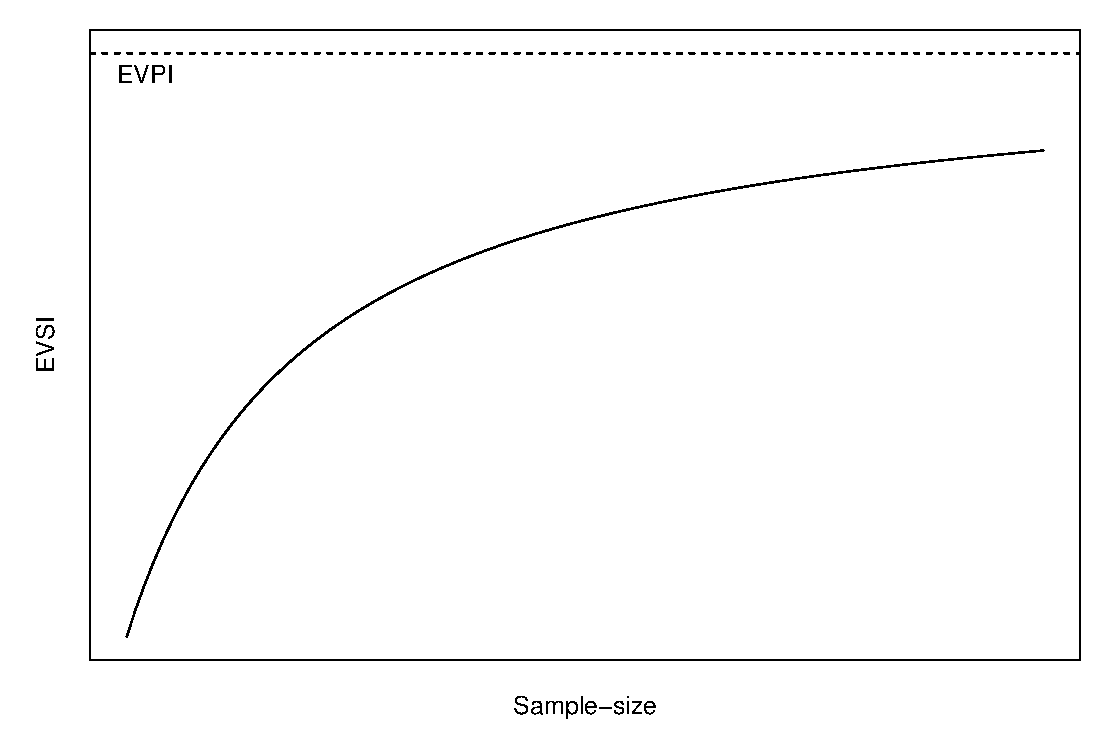
\includegraphics{voiReview_files/figure-latex/dimretplot-1.pdf}
\caption{\label{fig:dimretplot}As sample-size increases the expected value of sample
information (EVSI) approaches EVPI asymptotically.}
\end{figure}

The discrepancy between informal and formal information value, and the
explanation we provide above, highlights an important point about
VOI---that it follows a law of diminishing returns. In other words, the
relationship between the amount of information you have and its
cumulative value is non-linear. As one approaches perfect information,
the upper limit of information value, the relationship asymptotes. The
performance gain one would expect when going from a highly uncertain
state to a less uncertain state, will be greater than decreasing
uncertainty by the same amount, but starting from a state of more
complete knowledge. This relationship can be explained graphically if we
examine how the EVSI changes as we increase sample-size
(\ref{fig:dimretplot}). As sample-size increases the EVSI increases at a
diminishing rate such that for very large sample-sizes it approximates
EVPI, though it can never exceed it \citep{Raiffa1961}.

An important aspect of valuing information is all but missing from the
case-studies found in this review---the cost of acquiring new
information. For a value of information analysis to be ultimately of use
to a decision maker, the value of information must be compared to its
cost. Further, the cost and value must measured in the same units.
Either the value of information must be converted into the currency with
which information cost is being measured (dollars, time, etc.), or the
cost must be converted into the units of measurement of the decision
objective. Only when this conversion has been performed can a decision
maker really know if it is worthwhile collecting any knew information
and how much new information to collect. If the cost is equal to, or
exceeds the benefit expected from having it, then it should not be
collected and decision making should proceed with the current level of
uncertainty.

However, at the current time, these final steps in the process of
information valuing are missing from the conservation and resource
management literature. We found no cases of formal VOI analyses where
costs were presented. Only in a few cases was this done in the informal
branch. In most cases the cost was not presented in the same units as
the value of information \citep{Grantham2008, Grantham2009, Moore2010}.
The exception being \citet{Balmford1999} who found that the cost of
information was typically less than 0.7\% of the expected performance
under uncertainty, while the value of information was at least an order
of magnitude larger. Similarly, \citet{Nygard2016}, in their assessment
of the Finnish marine biodiversity monitoring program, assessed that
while the expected benefit of information was 50 to 150 million euros,
the cost was only 5.9 million. The lack of information about cost,
especially in the formal branch of VOI analyses represents a significant
gap in understanding. However, it is understandable that costing
information is relatively rare. First, formal VOI analyses propose
hypothetical future information collection, the cost of which must be
based on assumptions. Second, if the costs can be pinned down at all,
they must be converted to the same units as the management objectives
(or vice versa). This conversion is fraught, as very often managers are
reluctant to express their objectives (e.g., number of individuals of a
threatened species protected) in the same units that express their
management costs.

An important aspect of VOI analysis to consider is that it only capable
of valuing information in the context of the uncertainty characterized
by the system model of the decision problem it is applied to. So-called
black swans, or unknown unknowns \citep{Wintle2010}, cannot be accounted
for in formal VOI analysis \citep{Runge2011a}. Relatedly, one cannot
completely discount the serendipitous or extrinsic value of information.
That is, information doesn't exist in a vacuum, and information
collected for the purposes of increasing the performance of a particular
decision may be as helpful or even more so, in the context of a
completely different decision. These two issues show that to rely on the
formal decision theoretic definition of information value alone, may
under-value information and that it cannot be the only factor relied on
to decide whether information should be collected or not.

\bibliography{voiReview.bib}

\newpage
\begin{landscape}
\section*{Appendix B: Case studies in VOI for conservation and natural resource management}
\addcontentsline{toc}{section}{Appendix B: Case studies in VOI for conservation and natural resource management}

\subsection*{Table B1: Formal VOI}
\bgroup
\linespread{1}\scriptsize
\extrarowsep=_2mm^2mm
\begin{longtabu} to 230mm {|X[1,l] X[1,l] X[1,l] X[1,l] X[.8,l] X[1,l] X[1,l] X[1,l] X[1,l] X[1,l] X[1,l]|} \hline 
Case study & Subfield & System & Spatial Scale & Time Scale & Objective & Actions & Model & Uncertainty & Optimization & VOI \\ \hline
Kuikka etal, 1999 & Fisheries management & Baltic cod (\textit{Gadus morhua}) fishery & 1,600,000 km$^2$ & 1yr & Maximize yearly catch and minimize risk of recruitment failure & Choose catch effort & Age-structured stochastic population model & Represented by the probabilities that one of three different recruitment models applies to the fishery dynamics & Monte Carlo simulations & 3-7\% \\
Mantyniemi etal, 2009 & Fisheries Management & North Sea herring (\textit{Claupea harengus}) fishery & 570,000 km$^2$ & 20yrs & Maximize fishery profit over 20yrs & Choose catch effort & Bayesian stochastic population model & Alternative model structure: compensatory (Beverton-Holt) or over-compensatory (Ricker) density-dependence in survival of spawned eggs & Non-exhaustive brute-force search & 5\% \\
Costello etal, 2010 & Fisheries Management & Southern California Bight fishery & 11,000 km$^2$ & 1yr & Maximise the value of the fishery subject to a conservation weighting & Choose among candidate areas to include in reserve system and/or set a catch limits in candidate areas  & Metapopulation model & A set of 8 plausible dispersal kernels for the metapopulation model each kernel is equally likely to be the true kernel & - & 0-11\% \\
Moore etal, 2011 & Invasive species control & \textit{Acacia paradoxa} invasion of South Africa & 3 km$^2$ & 20yrs & Minimize costs and losses from invasion & Choose whether to contain, eradicate or take no action & Constant rate of spread from initial infestation to maximum possible extent defined by bioclimatic niche model & The extent of infestation is unknown & Numerical optimisation of non-linear simultaneous equations & 8\% \\
Runge etal, 2011 & Threatened species recovery  & Recruitment dynamics of Eastern migratory whooping crane (\textit{Grus americana}) population & 200 km$^2$ & 10yrs & Maximise number of breeding pairs, reproductive success, adult survival and condition & Choose among 7 separate management strategies  & Expert elicited hypotheses & Each hypothesis weighted according to expert opinion & Calculation of all terminal utilities for each combination of management action and hypothesis  & EVPI = 20\%, EVPXI = 1-11\% \\
Moore and Runge, 2012 & Invasive species control & Grey willow (\textit{Salix cinerea}) invasion of alpine bogs of the Bogong High Plains, Australia & 120 km$^2$ & 200yrs & Protect the integrity and function of alpine bogs & Allocate effort to control willows among 4 zones & State-based dynamic model & Probability distributions of model parameters & Monte Carlo simulations & EVPI = 0-10\%, EVPXI = 0-3.5\% \\
Johnson etal, 2014a & Wildlife harvest management & Dynamics of Svalbard population of Pink-footed Goose (\textit{Anser brachyrhynchus}) & 450,000 km$^2$ & 1yr & Maintain population size around 60,000 minimizing the probability that population collapses or erupts  & Choose harvest rate each year & Stochastic population model & Set of 9 structurally different population models & Stochastic dynamic programming & EVPI = 3-6\%, EVPXI = 0-2\% \\
Johnson etal, 2014b & Wildlife harvest management & Dynamics of Webb Wildlife Management Area Population of Northern Bobwhites (\textit{Colinus virginianus}) & 30 km$^2$ & 1yr & Maximise population growth rate, harvest, feasibility of management while minimizing cost. & 10 alternative management strategies with varying combinations of harvest rate, hunting practice, burn scale, food provision and water management & Stochastic population model & 4 different hypotheses of what is causing decline in population  & Calculation of all terminal utilities for each combination of management action and hypothesis  & EVPI = 3.5\%, EVPXI = 0-2\% \\
Canessa etal, 2015 & Threatened species recovery  & Survival of captive-bred and released European pond terrapins (\textit{Emys orbicularis}) in Liguria, Italy. & 5,500 km$^2$ & >3yrs & Maximise the survival of released individuals & Release terrapins at either 3, 4 or 5 years of age & Post release mortality rate that may vary by age. & Post release mortality may increase, decrease with age or is invariant & Calculation of all terminal utilities for each combination of management action and hypothesis  & EVPI = 6\% \\
Maxwell etal, 2015 & Threatened species recovery  & Dynamics of southeast Queensland population of Koala (\textit{Phascolarctos cinereus}) & 400 km$^2$ & >1yrs & Maximise population growth & Allocate budget to preventing  vehicle collisions, preventing dog attacks or restoring habitat & Age-structured population model & Structural uncertainty in the form of 8 different model structures. Parametric uncertainty in the form of probability distributions (represented by Monte Carlo simulations) of survival and fecundity & Multidimensional unconstrained nonlinear optimisations. & EVPI = 0-4\% \\
Williams and Johnson,  2015 & Wildlife harvest management & Dynamics of Svalbard population of Pink-footed Goose (\textit{Anser brachyrhynchus}) & 450,000 km$^2$ & 1yr & Maintain population size around 60,000 minimizing the probability that population collapses or erupts  & Choose harvest rate each year & Stochastic population model & Set of 9 structurally different population models & Stochastic dynamic programming & \\
Robinson etal, 2016 & Wildlife harvest management & White-tailed deer (\textit{Odocoileus virginianus}) population dynamics of New York, USA. & 140,000 km$^2$ & 1yr & Maximise hunting and minimize probability that population exceeds desired size & Six management altenatives: status quo, one buck bag limit, mandatory antler restrictions, partial mandatory antler restrictions, shorter seasons, voluntary restraint & Expert elicited predictions and population growth model & Parametric uncertainty for survival rates for different ages and each sex. Structural uncertainty represented by the inclusion or not of density dependent survival. & Calculation of all terminal utilities for each combination of management action and hypothesis across the range of parametric uncertainty & 0\% \\
\hline
\end{longtabu}
\egroup

\newpage

\subsection*{Table B2: Informal VOI}
\bgroup
\linespread{1}\scriptsize
\extrarowsep=_2mm^2mm
\begin{longtabu} to 230mm {|X[1,l] X[1,l] X[1,l] X[1,l] X[.8,l] X[1,l] X[1,l] X[1,l] X[1,l] X[1,l] X[.5,l]|} \hline 
Case study & Subfield & System & Spatial Scale & Time Scale & Objective & Actions & Model & Uncertainty & Optimization & VOI \\ \hline
Balmford and Gaston, 1999 & Spatial conservation planning & Country-wide reserve networks & 10,000,000 km$^2$ & > 10yrs & Establish a representative reserve system & Choose among candidate areas to include in reserve system & Assumption that selection rule criteria (intact vegetation, results of biodiversity surveys) predict success of reserve selected  & Represented as the information differential between simple selection rules and detailed biodiversity survey data & Unspecified complementarity-based spatial prioritization algorithm & >5\% \\ 
Grantham etal, 2008 & Spatial conservation planning & Proteaceous flora of the Fynbos biome, South Africa  & 81,000 km$^2$ & 10yrs & Maximally represent and retain proteaceous plant distributions in a reserve network & Choose among candidate areas to include in reserve system & Maximum entropy species distribution models of protea species in combination with simulation of vegetation loss and protection over time & Random subsets of complete dataset with sample-sizes ranging from, n = 100 (high uncertainty) to n = 44,000 (low uncertainty) And with the additional information provided by a habitat map. & Maximum gain and minimum loss greedy algorithms with convex square root benefit function (Zonation) & 2-24\% \\ 
Grantham etal, 2009 & Spatial conservation planning & Proteaceous flora of the Fynbos biome, South Africa  & 81,000 km$^2$ & 1-10yrs & Maximally represent and retain proteaceous plant distributions in a reserve network & Choose among candidate areas to include in reserve system & Maximum entropy species distribution models of protea species in combination with simulation of vegetation loss and protection over time & Similar to Grantham etal 2008, except instead random subsets, data was subsetted cumulatively through time & Maximum gain and minimum loss greedy algorithms with convex square root benefit function (Zonation) & <10\% \\ 
Moore and McCarthy, 2010 & Ecosystem restoration & Revegetation of Merri Creek Corridor, Melbourne, Australia & 400 km$^2$ & 20yrs & Maximise the area of successful revegetation over 20yrs/Maximise the number of 5-year periods in which there are at least 3ha of successful revegetation over 20yrs  & Allocating resources between planting at high (4000 plants/ha) or low (2000 plants/ha) density & The success of applying either action is stochastic and occurs with some probability unique to each.  & The probabilities that taking each action will be successful expressed as beta random variables & Stochastic dynamic programming & - \\ 
Stoms etal, 2011 & Spatial conservation planning & Farmland of the California Central Valley & 6300 km$^2$ & >1yrs & Maximise total benefits of Purchase of Development Rights program & Choose among candidate farms on which to purchase conservation easements & Benefits, Loss and Costs models predicting the payoff of an conservation easements scheme & Different data quality from datasets including, benefits only to benefits and costs and benefits, costs and losses. And minimal, basic, moderate and full information content & Rank farms by cost effectiveness and purchase until budget exhausted  & <2000\% \\ 
Baxter and Possingham, 2011 & Invasive species control & Red imported fire ant (Solenopsis invicta) invasion of Australia & 300 km$^2$ & 0.5 - 20yrs & Minimize density of Red imported fire ants & Choose which sites to search at and eradicate ants and choose whether to not search and just improve map of invasion & Logistic invasive spread model & Searchers are uncertain as to which sites within the invaded region are occupied according to maps of different quality & Stochastic dynamic programming & - \\ 
Hermoso etal, 2013 & Spatial conservation planning & Freshwater fish distribution of northern Australia & 1,200,000 km$^2$ & >10yrs & Minimize cost of set of planning units that protects at least 10\% of each species distribution & Choose among candidate areas to include in reserve system & Species distribution models (MARS) & Different data quantities 15 to 85\% subsets of full dataset & Spatial prioritisation algorithm (Marxan) & <230\% \\
Runting etal, 2013 & Spatial conservation planning & Coastal wetland communities of south-east Queensland, Australia. & 600 km$^2$ & 100yrs & Maximize the conservation value of purchased planning units & Choose among candidate areas to include in reserve system & Coastal impact model/Sea level rise projection & Combinations of coarse vs fine scale elevation data and a simple vs complex impact model forms a gradient of uncertain predictions & Maximum gain greedy algorithm with core area benefit function (Zonation) & 0-300\% \\
Perhans etal, 2014 & Timber harvest management & Silvicultural dynamics of Swedish Boreal Forests & 0.2 km$^2$ & >4yrs & Maximise the richness of lichen species and maximise the representation and richness of lichen species of conservation concern on retained aspen & Select among candidate aspen trees to retain  & Generalised linear models predicting biodiversity value of lichens on retained trees based on tree attributes & 4 different datasets used to produce selection criteria of varying uncertainty & Integer linear programming / selecting top ranked trees & - \\ 
Hermoso etal, 2015 & Spatial conservation planning & Freshwater fish distribution of northern Australia & 1,200,000 km$^2$ & >10yrs & Minimize cost of set of planning units that protects at least 10 or 25 or 50\% of each species distribution & Choose among candidate areas to include in reserve system & Species distribution models (MARS) & Systematic vs random sampling strategy & Spatial prioritisation algorithm (Marxan) & - \\ 
Lehtomäki etal, 2015 & Spatial conservation planning & Managed boreal forest of southeastern Finland & 14,000 km$^2$ & >4yrs & Maximise the representation of the spatial plan at minimal cost & Choose among candidate areas to include in reserve system & Expert elicited model relating biomass to ecological features of conservation value & Coarse vs fine scaled forest inventory datasets & Maximum gain greedy algorithm with additive benefit function (Zonation) & - \\ 
Mazor etal, 2016 & Spatial conservation planning & Loggerhead turtle (Caretta caretta) migration in the Mediterranean Sea & 2,500,000 km$^2$ & >1yr & Establish a reserve system that represents the entire life-cycle of migrating turtles at minimum cost & Choose among candidate areas to include in reserve system & Assumption that the datasets use represent the migration patterns of the turtles & Four different data-types of decreasing uncertainty: broad distribution, habitat types, mark-recapture data, telemetry data & Spatial prioritisation algorithm (Marxan) & - \\ 
Nygård etal, 2016 & Ecosystem management & Finnish marine biodiversity & 10,000 km$^2$ & 6yrs & Maximize the benefit of the program of measures & No management, intermediate management, strict management  & -  & Three scenarios: No information, indicative information, good information & -  & 50-151 million euro \\ 
Tulloch etal, 2016 & Spatial conservation planning & Kubulau District, Fiji, Fishery & 260 km$^2$ & >1yr & Minimize the cost of representing 30\% of the distribution of biodiversity features & Choose among candidate areas to include in reserve system & Assumption that various datasets represent the biodiversity value of the reserve system & Coarse and fine-scale input data & Spatial prioritisation algorithm (Marxan / MarProb) & - \\ 
\hline
\end{longtabu}
\egroup

\end{landscape}


\end{document}
